\section{Corpora}
%GATE Teamware provides means to perform operations in a remote GATE Datastore.

\subsection{Corpora List}\label{section:corpora-list}
To view existing corpora, choose \emph{Resources $>>$ Documents} from the top
menu. New page will be shown with the complete list of available corpora as
shown in Figure ~\ref{fig:corporalist}.
\begin{figure}[htb]
\centering
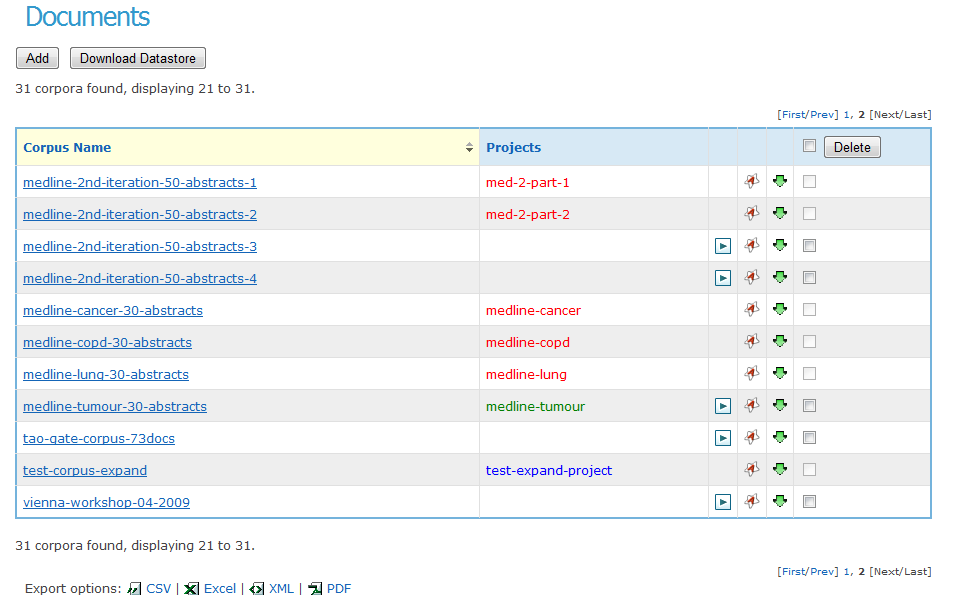
\includegraphics[scale=0.4]{corporalist}
\caption{Copora List}
\label{fig:corporalist}
\end{figure}
From this page, you can choose several
options:
\begin{description}
\item [Modify Corpus] To view details about already existing corpus, click on
the link showing the corpus name, or the first icon in the row. If you want to
add some new documents in corpus, you can do this by clicking on
\emph{Upload Documents} button.
\item [Start Annotation Project] Directly from the corpora list, you can start
annotation project for each corpus, by clicking on the \emph{start} icon. 
The annotation projects will be
explained in details in the next chapter. For now, have this option in mind as
a convenient way to start annotation from this page.

\item [View Annotation Projects] You can see if some annotation project is
running, suspended or finished over each corpus. The links to the annotation
project statistics can be of different colours, depending on project status:
\emph{red}: suspended; \emph{blue}: running; \emph{green}: completed. More about
project statistics you can find in the next chapter.

\item [Download Corpus] If you click on \emph{Download} link (second icon from
the right) you will download the corpus with all documents in it, archived in
zip file.
\item [Download Datastore] If you click on \emph{Download Datastore} button you
will download whole datastore with all corpora, archived as zip file.
\item [Delete Corpus] If you tick the checkbox in \emph{Delete} column (last
column on the right hand side) and press \emph{Delete} button you will delete
selected corpora with all documents in them.
\end{description}

\subsection{Create Corpus}
To create a new corpus, click on the \emph{Add} button on the corpus list page.
New window will open (see Figure ~\ref{fig:addcorpus}). Specify the corpus name
and encoding. By default the
encoding is UTF-8 which should be fine for most of the documents. However if
you need some particular encoding, you should specify it here. Click
\emph{Browse} button to provide the full path of your zip archive from your file
system.

\begin{figure}[h]
\centering
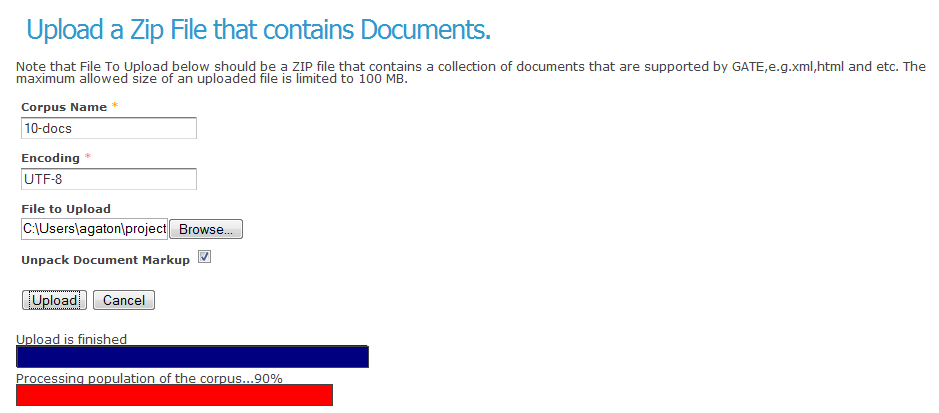
\includegraphics[scale=0.5]{populatecorpus}
\caption{Add Corpus }
\label{fig:addcorpus}
\end{figure}

GATE Teamware will try to identify the type of the document, then strip
and convert any markup into GATE's annotation format. To disable this process,
uncheck the option \emph{Unpack Markup Aware}. Finally click on the
\emph{Upload} button to populate the corpus.

Please have in mind the following conditions:
\begin{itemize}
\item documents need to be packaged in zip archive
%You have nested folders in zip archive.
\item documents have to be in a format supported by GATE:
Plain Text, HTML, SGML, XML, RTF, PDF, DOC or XLS
	
\end{itemize}
\begin{figure}
If the corpus is populated successfully, you should see a screen similar to the
one shown in Figure \ref{fig:corpuspopulated}.
\centering
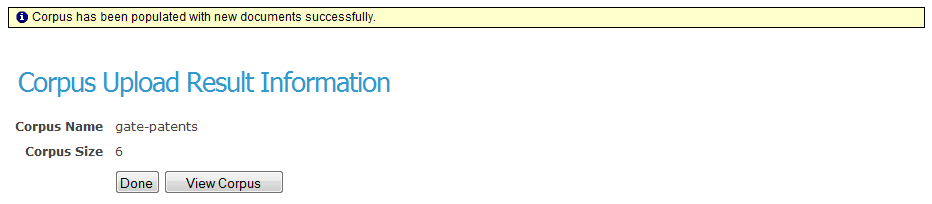
\includegraphics[scale=0.4]{corpuspopulated}
\caption{Corpus created}
\label{fig:corpuspopulated}
\end{figure}

Please make sure that the zip archive you are uploading is created by standard
zip archiver tool and that compression method used is
DEFLATE\footnote{\url{http://en.wikipedia.org/wiki/DEFLATE}}. There should be no
problem with standard zip implementation under Windows and Unix.
In case you get the error message like in Figure
\ref{fig:unsupportedcompressionmethod},
try to zip your corpus with the different tool.
\begin{figure}
\centering
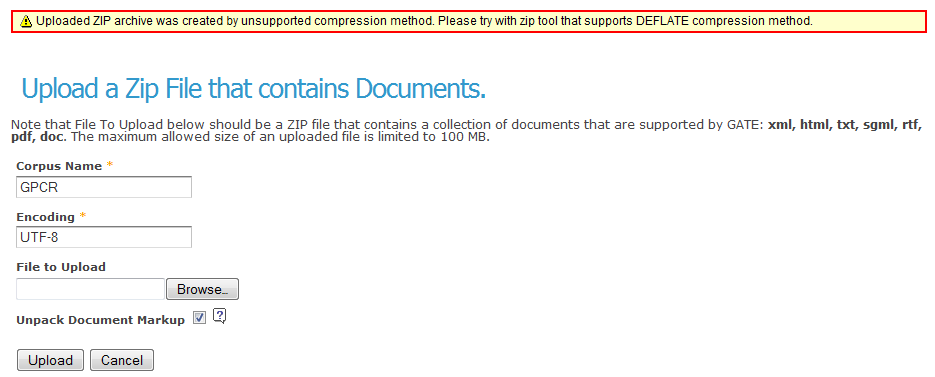
\includegraphics[scale=0.4]{unsupportedcompressionmethod}
\caption{Unsupported Compression Method}
\label{fig:unsupportedcompressionmethod}
\end{figure}

\subsection{ANNIC Search}
To use ANNIC Search facility, click on the ANNIC icon for the corpus you want
to carry out the search. A Java Web Start application - ANNIC GUI will be
activated. 

\begin{figure}[hb!]
\centering
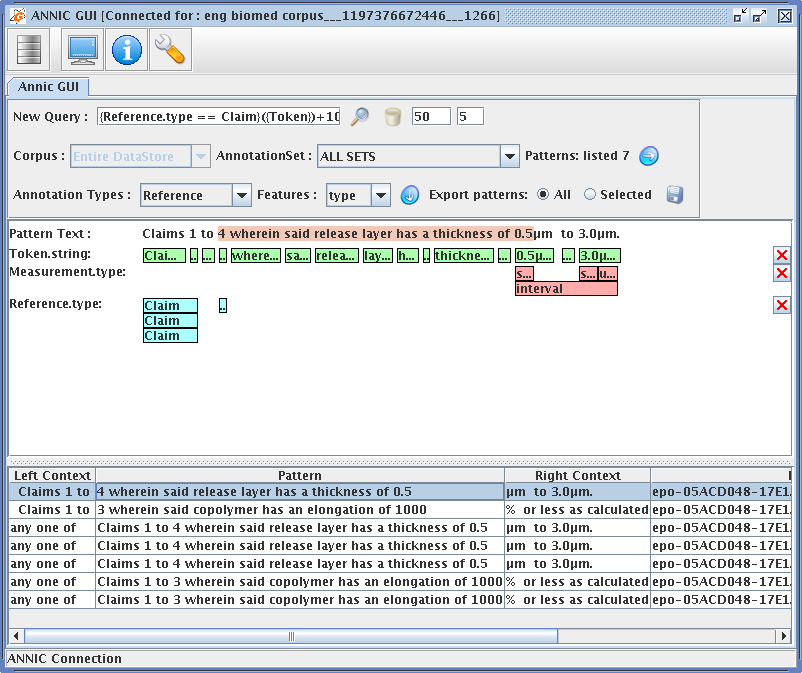
\includegraphics[scale=0.4]{annicresult}
\caption{Annic Search Result}
\label{fig:annicresult}
\end{figure}

The Figure  ~\ref{fig:annicresult} shows ANNIC
in action. Since ANNIC allows indexing documents
with annotations and features, the syntax of ANNIC query contains LHS part
of the JAPE pattern/action rule.



For example, the query:
${Reference.type == Claim}({Token})+10{Measurement}$ will find first an
annotation of type \emph{Reference} that has a feature named type with the value
\emph{Claim}, then to allow from 1 to 10 annotations of type \emph{Token}, i.e.
a word or punctuation, and eventually to find an annotation of type
\emph{Measurement}. This query can be interpreted as a search for finding a
reference to a claim that involve measurement.

To execute a query, enter it in the query text field, and click
on the magnifying glass icon. You can choose annotation sets,
then the annotation type, and features to add to the middle part of the
GUI with the bottom arrow icon. If there is more than one page of results
you need to use the right arrow icon to see the next page of results.

You can see the results in the bottom part of the GUI that lists in a
table the matching patterns, their contexts, the name of the document
and annotation set. In the middle part, you can see the annotations
and features with their values for the line selected in the bottom part.

Help window is provided in the GUI if you click on the information
sign icon in the top tool bar. For more information about Annic and JAPE, please
check Gate User Guide.

\section{Documents}
\subsection{Document list}
To see the list of documents inside the corpus click on \emph{View} link next
to the corpus name. New page will open as shown in
Figure ~\ref{fig:documentlist}.
\begin{figure}[h]
\centering
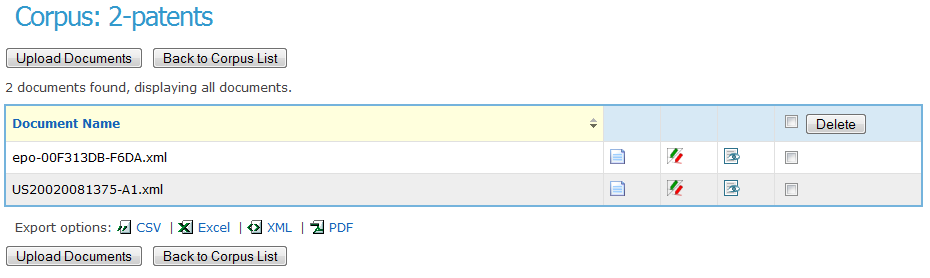
\includegraphics[scale=0.5]{documentlist}
\caption{Document List}
\label{fig:documentlist}
\end{figure}

To delete a document from the corpus, simply tick the checkbox next to document
and click on the
\emph{Delete button}. You can choose to delete all listed documents by ticking
the box from the top of the table.

\subsection{View Document with Annotation Editor}\label{section:annotation-editor}
To open/edit a specific document, click on the \emph{View Document} icon (the
first icon from the left hand side shown in Figure~\ref{fig:documentlist}).
Annotation Editor will be activated and start
loading the document. As shown in Figure ~\ref{fig:annotatorgui}, users can
now carry out the annotation tasks within the Annotator GUI.

\begin{figure}[ht!]
\centering
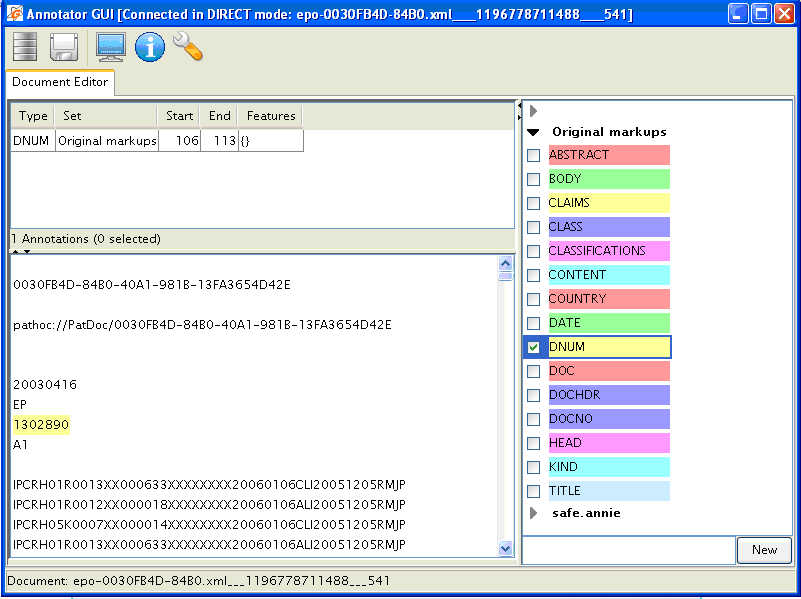
\includegraphics[scale=0.35]{annotatorgui}
\caption{Annotation Editor}
\label{fig:annotatorgui}
\end{figure}

\subsection{Compare Annotations with Annotation Differ}\label{section:annotation-differ}

To use the Annotation Differ facility on the document, click on the icon
\emph{Annotation Differ} on the documents list page (the second icon from the
left hand side shown in Figure ~\ref{fig:documentlist}). Then, you should see the
Annotation Diff Editor, where you need to specify which two annotation sets
and the common annotation type you want to compare.

\begin{figure}[hb!]
\centering
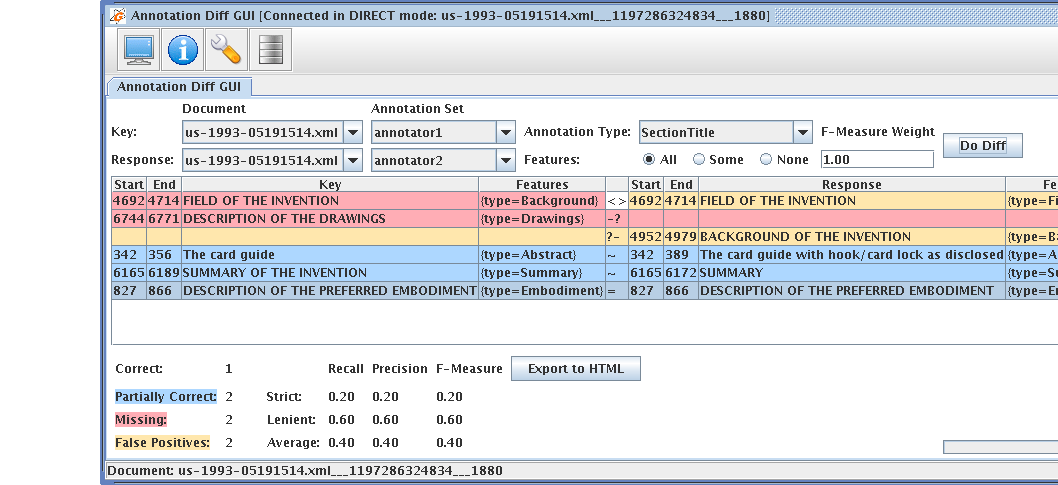
\includegraphics[scale=0.32]{anndiffgui}
\caption{AnnDiff Editor}
\label{fig:anndiffgui}
\end{figure}

Figure ~\ref{fig:anndiffgui} depicts a comparison
between two annotators who have their annotations contained respectively in
\emph{annotator1} and \emph{annotator2} annotation sets. The first is the key,
i.e. the gold standard, and the second is the response, i.e. the tested data.
There is a common annotation type \emph{SectionTitle} in these annotation sets.
It is thereby possible to do a comparison on this annotation type.

The option \emph{Features} has been set on \emph{All} -- this means that all
values of the
features are taken into account during comparison. For example, the first
line in the table shows for the same text, \emph{Field of invention}, two
different feature values, \emph{Background} and \emph{Field} for the same
feature named \emph{type}.

You can see different colors according to the type of difference between the
annotations from each annotation set that is also shown in the central column
of the table.

Help window is provided in the GUI if you click on the information sign icon
in the top tool bar. For more information, please refer to the \emph{Chapter 13},
Performance Evaluation of Language Analysers, in Gate User Guide
(\url{http://www.gate.ac.uk/sale/tao/index.html}).

\subsection{IAA Calculation}
From the document list page, you can do IAA calculation over annotation sets on
each document. Click on the IAA icon (third icon from the left hand side shown
in Figure~\ref{fig:documentlist}), and the new page should open as shown in
Figure~\ref{fig:iaacalculation}.
\begin{figure}[ht!]
\centering
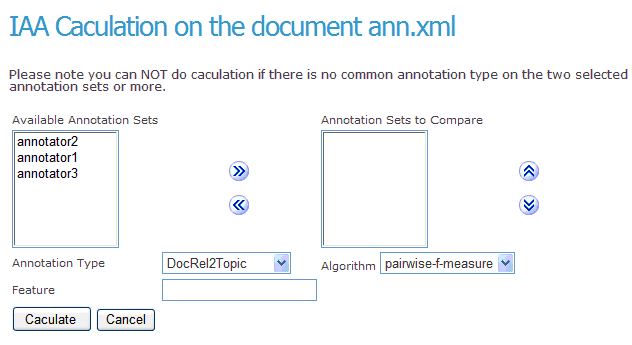
\includegraphics[scale=0.4]{iaacaculation}
\caption{IAA Calculation}
\label{fig:iaacalculation}
\end{figure}

You need to select at least two annotation sets from the left available
annotation sets box and move them to the right box to do the comparison over a
shared annotation type. Also there are four algorithms available for you to choose.
The screenshot shown in Figure ~\ref{fig:iaaresult} is an example of the result
based on the chosen annotation sets, type and algorithm. Note: four algorithms
offer different result formats because of their difference in various values.

\begin{figure}[h!]
\centering
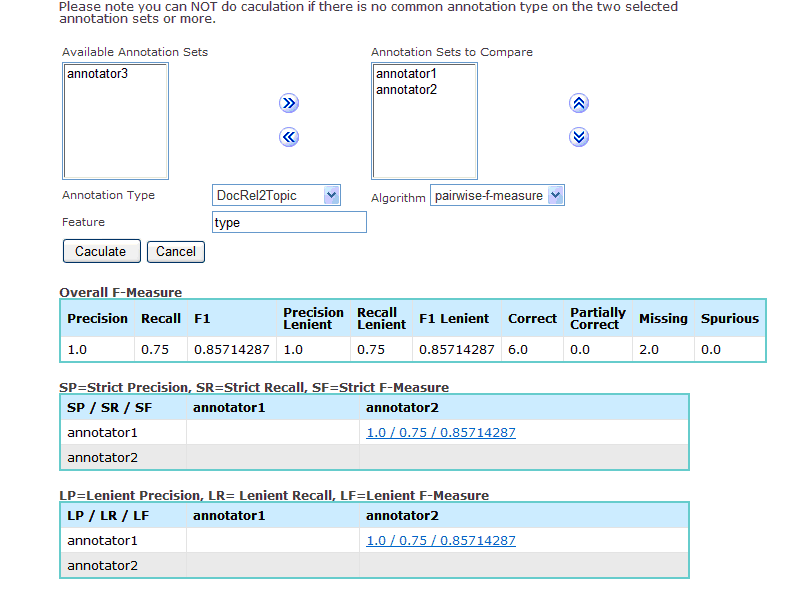
\includegraphics[scale=0.4]{iaaresult}
\caption{IAA Calculation Result}
\label{fig:iaaresult}
\end{figure}

\clearpage